%%%%%%%%%%%%%%%%%%%%%%%%%%%%%%%%%%%%%%%%%%%%%%%%%%%%%%%%%%%%%
%% HEADER
%%%%%%%%%%%%%%%%%%%%%%%%%%%%%%%%%%%%%%%%%%%%%%%%%%%%%%%%%%%%%
\documentclass[a4paper,oneside, titlepage, 12pt]{article}
\usepackage{fancyhdr} %%Fancy headings

\usepackage[cp1251]{inputenc}
%% Language %%%%%%%%%%%%%%%%%%%%%%%%%%%%%%%%%%%%%%%%%%%%%%%%%
\usepackage[USenglish, russian]{babel}
\usepackage[T2A]{fontenc}

\usepackage{graphicx} %%For loading graphic files
%\usepackage{longtable} %%For tables, that exceed one page
%% Other Packages %%%%%%%%%%%%%%%%%%%%%%%%%%%%%%%%%%%%%%%%%%%
\usepackage{a4wide} %%Smaller margins = more text per page.
\usepackage{color}
\usepackage{colortbl}
\usepackage[pdftex, unicode, colorlinks, linkcolor=black, urlcolor=blue]{hyperref}

\begin{document}
\uchyph=0
\hfuzz=1pt

\newpage
\title{
	\textcolor[rgb]{.67,.05,.05}{Knowledge} \textcolor[rgb]{.23,.62,.25}{Base} source \textcolor[rgb]{.11,.45,.86}{Editor} 					\\version 0.3.0 (intergator)
	
\includegraphics[]{../images/title.png}
}
\author{Харкунов Евгений \and Корончик Денис}
\date{4 мая 2012}
\maketitle

\pagestyle{empty}
\tableofcontents
%\newpage
%%%%%%%%%%%%%%%%%%%%%%%
% Colontitul settings %
%%%%%%%%%%%%%%%%%%%%%%%
\pagestyle{fancy}
\lhead{\sectionmark}
\chead{}
\rhead{\thepage}
\lfoot{Copyright OSTIS 2010-2012 \copyright}
\cfoot{}
\rfoot{www.ostis.net}
\renewcommand{\headrulewidth}{0.9pt}
\renewcommand{\footrulewidth}{0.9pt}

\section{��������}

\textit{Knowledge Base source Editor} �������� �����������, ������� ���������� �� ������ � �������� � �������������� ���������� ��� ������ ���������������� ������, �������������� ������� �������� �� ���������� \textbf{OSTIS}. � ������ ������� ��������� ������� ������� ������������ ������, ���������� � ���� ������, ��� ������� �������� ������� �� �������������� � �������� ������� �������������� ��� ������.

P.S. ����������� �������������� � ������ �����������:
\begin{itemize}
	\item
		
\includegraphics[width=30px, height=30px]{../images/lamp.png}
 - ����������, ������ ����������.
	\item 
		
\includegraphics[width=30px, height=30px]{../images/note.png}
 - �������, �������������� �����������.
\end{itemize}
 



\section{���������}

��������� ����������:
\begin{itemize}
	\item ������������ �������: Linux/Mac/Windows
\end{itemize}

\subsection{Windows}

����� ���������� ����� ������ ��������� ������� ��� ���\-������� ������.
��� ��������� ���������� ��� ���������� ������� ����������� � \href{http://sourceforge.net/projects/ostis/}{�����} �������.
����� �������, ��������� ���� �����, ���� �� ���������� ��� ����������� ��������� ���������.

��� ������������ ������� ���������� �������� \textbf{���� -> ��������� -> KBE -> KBE}.

\subsection{Linux \& Mac}

���� ������������ ������ �������� ������� ������ ��� linux � ��� ������� � �� ����������. �������� ���� ��������� �� ������: \href{http://github.com/deniskoronchik/kbe}{http://github.com/deniskoronchik/kbe}
� ����� {\tt sources} ��������� ������ {\tt kbe.pro} ��� \textit{QtCreator}.
\section{����������� ���������}

������ ��� ���������� � ����������� ���������, ���������, ��� ������� ����� �������� �� ���� ������� � ������ �����������.

\begin{itemize}
	\item ���� �� ���������� �����-���� ������, �������� �� \href{http://www.ostis.net/forum/viewtopic.php?f=8&t=283}{������} � �������� ������� ��������� ��������.
	\item ���� � ��� ��������� ���� �� ��������� ���������, �� ���� ����� �� ������ �������� �� \href{http://www.ostis.net/forum/viewtopic.php?f=8&t=86}{������}.
\end{itemize}

\section{�������� �������������� ��������}

�� ������ ������ KBE ��������� ������������� ���������� ���������� � ��������� ��������:
\begin{itemize}
	\item {\tt GWF} � ������ ��� �������� sc.g-�����������
\end{itemize}

��� ������������� ����������� ����� ���� �������������� � ��������� ������� �����������:
\begin{itemize}
	\item {\tt BMP} - Windows Bitmap
	\item {\tt ICO} - Windows Icon
	\item {\tt JPEG}, {\tt JPG} - Joint Photographic Experts Group
	\item {\tt PNG} - Portable Network Graphics
	\item {\tt PPM} - Portable Pixmap
	\item {\tt SVG} - Scalable Vector Graphics
	\item {\tt TIF}, {\tt TIFF} - Tagged Image File Format
	\item {\tt XBM} - X11 Bitmap
	\item {\tt XPM} - X11 Pixmap
	\item � ��.
\end{itemize}

\section{�������� ����������}

\subsection{������� ���� ����������}
\begin{figure}[h]
	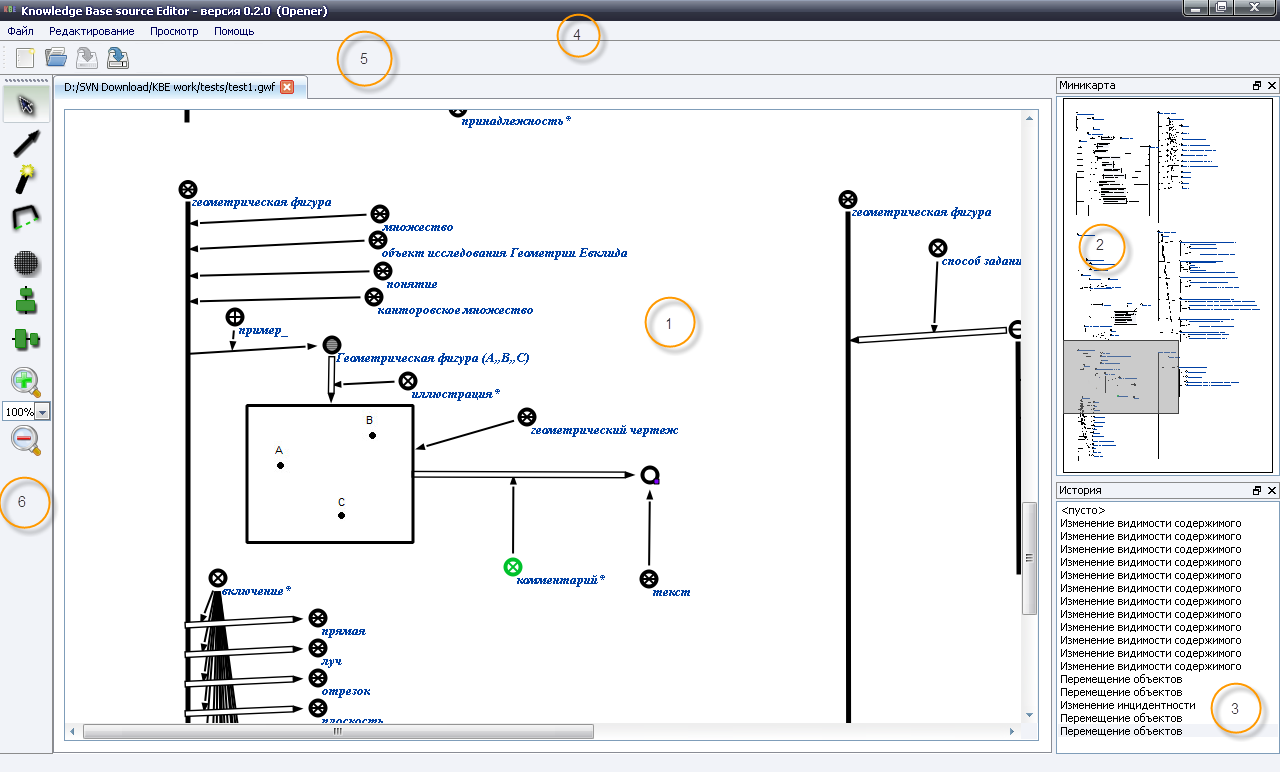
\includegraphics[width=16.23cm, height=9.82cm]{../images/mainwindow.png}
	\caption{������� ���� ����������. 1 � �������� ������� �������; 2 � ���������; 3 � ������� ��������� � �������� �������� 				���������; 4 � ������ ����; 5 � ������� ������ ������������; 6 � ������ sc.g-������������.}
	\label{mainwindow}
\end{figure}
������� ���� ���������� ������������ ����� ��������� ����� ������� � ������������, ������� ����� ����� ����������, �������� ���� ����������� ����������.

\subsubsection{�������� ������� �������}

�������� ������� ������� ������������� ������������ ������������, ��������� �� ���������� �������, ���������� ������� ������������� ���������� �������� �� ������� ������ ����������. ������ ������� �������� ���������� �������� ������� ���� ������ �������������� �� ��������� ������� �����. �������� �������� �������� � ��������� ������� ������� ��. � �������~\ref{usage}.

\subsubsection{��������� � ������� ���������}

��������� ������������� ��� ������ � ������� ��������� �� ��������� ���������. ������� ��������� ��������� ��������� ������������ �������� � ���������� ��������, ������� �� �������� � ���� �������������� ���������.

\hrule\smallskip
\noindent
\includegraphics[width=25pt, height=25pt]{../images/lamp.png} \textcolor[rgb]{.25, .67, .2}{\textbf{����������}: ���� ����� ������ ������ �������� ���������� ����� ���� ��������, ��������� � ���������������, �� ���������� �������� ����� �������.}
\smallskip
\hrule

\subsubsection{������ ����}

������ ���� �������� �������� ������� ��� ������ � �����������.
\begin{figure}[h]
	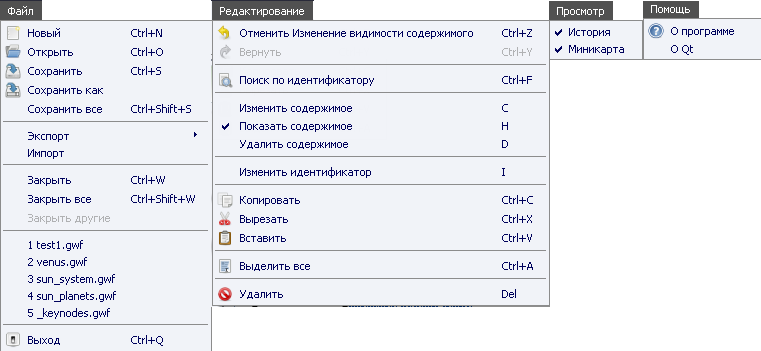
\includegraphics[width=16.22cm, height=7.51cm]{../images/menus.png}
	\caption{�������� ���� ����������.}
	\label{menus}
\end{figure}

\hrule
\smallskip
\noindent
\includegraphics[width=25pt, height=25pt]{../images/lamp.png} \textcolor[rgb]{.25, .67, .2}{\textbf{����������}: ���� �\textbf{��������������}� ����� ��������� �������� � ����������� �� ���������� �� ������ ������ ��������. ����� ��� �������� ����������� ����������� ���� ������� (����������� �� ������� ������ ������� ���� �� �������).}
\smallskip
\hrule

\subsubsection{������� ������ ������������}
�������� �������� ��������, ����������� ��� ��������� ��������� ���������.
\begin{figure}[h]
	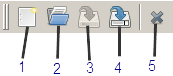
\includegraphics[width=5.72cm, height=2.57cm]{../images/maintoolbar.png}
	\caption{������� ������ ������������. 1 � �������� ������ ���������; 2 � �������� ��� ������������� ���������; 3 � ��������� 		������� ��������; 4 � ��������� ������� �������� ���; 5 - ������� ������� ������� .}
	\label{maintoolbar}
\end{figure}
\section{�������������}
\label{usage}

��� ������ ������� KBE �� ������ ���������, ��� ����� ��������, �������� � ������� ������ ��� ������ ������ �� �������. ������ ������� ���������� �� ������ � �������� ���� ��������.

������ � ����� ���������� ���������� c �������� ������ ���������, ���� �������� ��� �������������.
\begin{enumerate}
	\item \textbf{��������}: M��� \textbf{���� -> �����}, ���� ������ �� 
\includegraphics{../images/document-new.png} ������� ������ ������������ (��. �������~\ref{maintoolbar}).
	\hrule
	\smallskip
	\noindent
\includegraphics[width=25pt, height=25pt]{../images/note.png} \textcolor[rgb]{.67,.05,.05}{������� ����� �������� ����� ��������� ��������� ������ \textbf{Ctrl+N}.}
	\smallskip
	\hrule

	\item \textbf{��������}: ����� ���� \textbf{���� -> �������}, ���� ������ 
\includegraphics{../images/document-open.png} �� ������� ������ ������������ (��. �������~\ref{maintoolbar}).
	\hrule
	\smallskip
	\noindent
\includegraphics[width=25pt, height=25pt]{../images/note.png} \textcolor[rgb]{.67,.05,.05}{������� �������� ����� ��������� ��������� ������ \textbf{Ctrl+O}.}
	\smallskip
	\hrule

	\item \textbf{����������}: ����� ���� \textbf{���� -> ���������} (\textbf{��������� ���}, \textbf{��������� ���}), ���� �������������� ������ �� ������� ������ ������������ (��. �������~\ref{maintoolbar}).

	\item \textbf{�������}: ����� ���� \textbf{���� -> �������}.
\end{enumerate}
\subsection{�������� sc.g-�����������}
��� �������������� ���������� ���������, � ������� SCg-����, �������� ��������� ���� sc.g-���������: {\sf sc.g-����}, {\sf sc.g-����}, {\sf sc.g-����}, {\sf sc.g-������}.
 
����� ��������� ������� �������������� sc.g-����������� �������� ��������� ������ ��������������. � ������ �� ����� ������� �������������� ������������ ����� ��������� ������� ������������� ����. �������� ������ �������������� � ����� ������ �������� �� ������ ������������. 
\begin{figure}[h]
	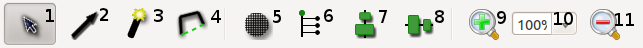
\includegraphics[width=15.77cm, height=1.27cm]{../images/scgtoolbar.png}
	\caption{������ ������������: 1 � ����� ���������; 2 � ����� �������� ���; 3 � ����� �������� ���; 4 � ����� �������� ��������; 5 � ������������ �� �����; 6 � ������������� ������ � �����; 
7 � ������������ �� ���������; 8 � ������������ �� �����������; 9 � ���������� ��������; 10 � ��������� �������� �������� ����������� �����; 11 � ���������� ��������.}
	\label{scgtoolbar}
\end{figure}

���������� ��������� ������ �������������� � �������, ������� �������� �� ������ ������������:
\begin{enumerate}
	\item ����� \textbf{��������� � ����������� ��������}. � ������ ������ ������������ ����� �������� �� ����� ��������� ������� ��, ��������� ��, ������� ����������� ���� � ���������. 
������������� ������������ ������� ������ �������� ��, ��� � ��� ����� ��������� {\sf sc.g-����}. ��� ����� ���������� ��������� ������� ���� ����� � �����, ��� ���������� ������� ���� (� ������ �������� ��� ���������� ���� �� ������ ���� ������ ��������);
	\item ����� \textbf{�������� ���}. �������� ���� ���������� � ����, ��� ������������ ��������� ������ �� �������� ��� ����� �������� (���� ����� ������� ����), ����� �� ����� ������� ����� ������ ���� (���� ����� ������� ����, � ������ ����� ���������), ����������� �������� ��������� ��������� ������� (���� ����� ������� ����). � �������� �������� ������������ ����� �������� ��������� �������� (�������� ���������� �������, ����� ������) ����� ����� ������ ������� ����;
	\item ����� \textbf{�������� ���}. ���� ������������ ��� ���������� ���������� ������� ����, ������� ��� ����� ����������� ���� ��� �����. �������� ���� ���������� � �������� ����, ��� ������� ��� ��������� (���� ����� ������� ����), ����� ��� � ��� �������� ��� ����������� ����� ������. ����������� �������� ���� ����� ����� �� ��������� ����� ������ (��� ��������� �� ���, �������� {\bf\it �������� �����}). ��� � ��� �������� ��� ������������ ����� �������� ��������� �������� �������� ������ ������� ����;
	\item ������ \textbf{�������� ��������}. �������� ������� ����������� � �������� ��� �����. ����������� ������� ������ ����� ������� ���� �� ��������� ����� (��� ��������� �� ��� ���������� �������� �����).  ��� � ��� �������� ��� � ��� ������������ ����� �������� ��������� �������� �������� ������ ������� ����;
	\item ������� \textbf{������������ �������� �� �����}. ������ ������� ��������� ��������� ������� ��������� � ��������� �� �����. ������� ����� ����������� ��� ������������� ������� � ������� ��������.
\begin{figure}[h]
	\centering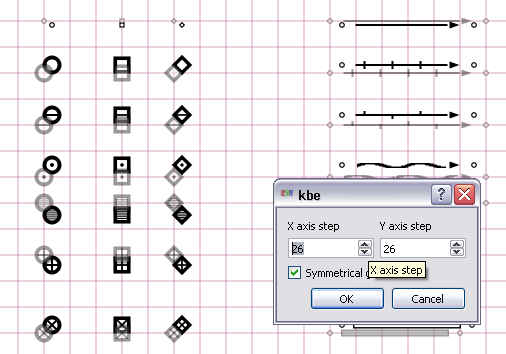
\includegraphics[height=10.98, height=5.75cm]{../images/gridaligment.png}
	\caption{������ ������������� ������� ������������ �� �����}
	\label{gridaligment}
\end{figure}
� ���������� ����, ������� ���������� ����� ������������� �������, ����� ���������� �������� ������� ����� (��. �������~\ref{gridaligment}).
	\item ������� \textbf{������������ ������ � �����}. ������ ������� ��������� ��������� ���� � �������� ������� ����, � ���������� (����������) ������. ��� � � ������ ������������ �� �����, ��� ������������� ������� ���������� ���� �������� (��. �������~\ref{tuplealigment}). ��� ������������� ������� ���������� �������� ���� �� �������� ������� ����.
	
\begin{figure}[h]
	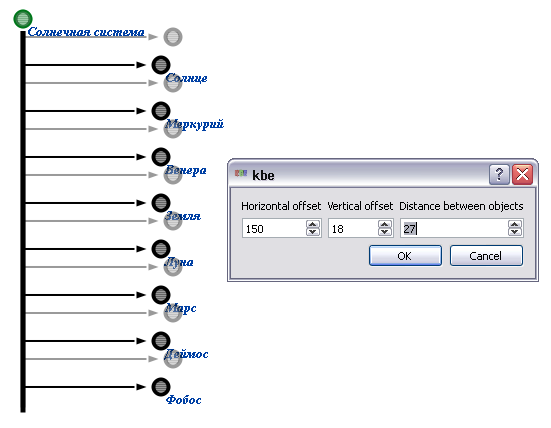
\includegraphics[width=13.07cm, height=9.82cm]{../images/tuplealigment.png}
	\caption{������ ������������� ������� ������������ ������ � �����}
	\label{tuplealigment}
\end{figure}
	\item ������� \textbf{������������ �� ������������ �����}. ������������� ������� �������� � ������������ �� X ���������� ���������� ��������. ����� ���������� ��������� ��� ������� �������������� X ��������� ���������� ��������. Y ���������� �������� �� ��������. ������� �� ����� ��������;
	\item ������� \textbf{������������ �� �������������� �����}. ������������� ������� �������� � ������������ �� Y ���������� ���������� ��������. ����� ���������� ��������� ��� ������� ���a���������� Y ��������� ���������� ��������. X ���������� �������� �� ��������. ������� �� ����� ��������;
	\item ������� \textbf{���������� ��������}. ������������� ������� �������� � ���������� �������� �����������;
	\item ������ \textbf{����������� ���������}. ������� ����������, ������� ��������� ������� ������� �� ��� ������� ���������, ���� ������� ���� �������;
	\item ������� \textbf{���������� ��������}. ������������� ������� �������� � ���������� �������� �����������.
\end{enumerate}

\hrule
\smallskip
\noindent
\includegraphics[width=25pt, height=25pt]{../images/note.png} \textcolor[rgb]{.67,.05,.05}{������ ����� ����� ������������ �������� ������ 1-4. ����� � ������� ������������ ��������� 5-8.}
\smallskip
\hrule
\smallskip
\hrule
\smallskip
\noindent
\includegraphics[width=25pt, height=25pt]{../images/note.png} \textcolor[rgb]{.67,.05,.05}{����������� ������������ ������������ �� ����� � ������ � �����. �������� �������� ������� ����� ��� ��������� ��� ����, �� ������ ��������� ������� ������� 5 � 6 ������ ������� �����������.}
\smallskip
\hrule
\medskip
����� ������������ ���� ������ ���������� ��� ����� ��� ������ ��������������:
\begin{itemize}
	\item ������� \textbf{��������� ��������� ���������� �������������� ��������}. ������ sc.g-�������� ����� ������������� ��������� ��������� �������������. ��� ����, ����� ���������� (��������) ��������� ������������� sc.g-��������, ���������� � ����������� ���� ������� �������� ������� ����� �\textbf{�������� �������������}�, ���� ��������������� \textit{������� ��������} \textbf{I}. ����� ���� ����� ������� ���������� ����, � ������� �� ������� ������ ����������� ������������� (��. �������~\ref{idtfdialog}).
	\begin{figure}[h]
		\centering
\includegraphics[width=6.70cm, height=3.92cm]{../images/idtfdialog.png}
		\caption{���������� ���� ��������� ���������� ��������������}
		\label{idtfdialog}
	\end{figure}
	\item ������� \textbf{��������� ���� ��������}. ��������� �������� ��� sc.g-�������� (�������������, ����������� ��� � �.�.). ��������� ���� ����� ������� �������� ������ ������� ���� �� �������� (��� �������� ����� ����������) � ������ ������� ���� � ���� \textbf{�������� ���};
	\item ������� \textbf{��������� �����������}. ���������� ���������� ��� sc.g-���� ���������� ������, ��� ����� ����������  ������ ������ �������� ���� �� ���� � ������� ������� ��������� �����������. ����� ������������� ������� ���������� ������, � ������� ����� ������� ��� ����������� � ���� ���������� (��. �������~\ref{contentdialog})
	\begin{figure}[h]
		\centering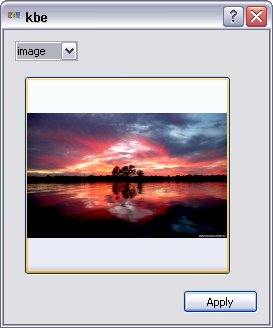
\includegraphics[width=6.09cm, height=7.46cm]{../images/contentdialog.png}
		\caption{������ ��������� �����������}
		\label{contentdialog}
	\end{figure}
	\hrule
\smallskip
\noindent
\includegraphics[width=25pt, height=25pt]{../images/lamp.png} \textcolor[rgb]{.25, .67, .2}{\textbf{����������}: ���� �������������� � ����� ������� ������ ��������� ����������� �� �����. ��� ����� ���� ���� ���������� ���� �� ����, ����� ���� ��������� sc.g-���� � ���������� �������� ����� ���������� ��������������� ����.}
\smallskip
\hrule
\end{itemize}

\section{������ ������� ������}

\begin{tabular}{|c|l|}
\hline
\textit{��������� ������} & \textit{����������} \\
\hline
\multicolumn{2}{|c|}{\textbf{������� ����}} \\
\hline
Ctrl+N & �������� ������ ��������� \\
\hline
Ctrl+O & �������� ������������� ��������� \\
\hline
Ctrl+S & ��������� ������� �������� \\
\hline
Ctrl+Shift+S & ��������� ��� �������� �� ������� ������ ��������� \\
\hline
Ctrl+W & ������� ������� ������� \\
\hline
Ctrl+Shift+W & ������� ��� �������� �������\\
\hline
\multicolumn{2}{|c|}{\textbf{���� ��������������}} \\
\hline
Ctrl+X & �������� \\
\hline
Ctrl+C & ����������\\
\hline
Ctrl+V & �������� \\
\hline
Ctrl+Z & �������� �������� \\
\hline
Ctrl+Y & ������� �������� \\
\hline
Ctrl+A & �������� ��� \\
\hline
Ctrl+F & ����� �� �������������� \\
\hline
\multicolumn{2}{|c|}{\textbf{������ SCg-������������}} \\
\hline
1 & ����� ���������\\
\hline
2 & ����� �������� SCg-���� \\
\hline
3 & ����� �������� SCg-���� \\
\hline
4 & ����� �������� SCg-������� \\
\hline
5 & ������������ �� ����� \\
\hline
6 & ������������ ������ � ����� \\
\hline
7 & ������������ �� ��������� \\
\hline
8 & ������������ �� ����������� \\
\hline
+ & ��������� ������� \\
\hline
- & ��������� ������� \\
\hline
\multicolumn{2}{|c|}{\textbf{����������� �����}} \\
\hline
Ctrl+������ ���� & ����������/���������� �������� ����������� ����� \\
\hline
Ctrl+������� & ����������� ������� \\
\hline
I & ��������� �������������� ������� \\
\hline
C & ��������� ����������� ���� \\
\hline
H & �����������/������� ����������� ���� \\
\hline
D & �������� ����������� ���� \\
\hline
Delete & �������� �������� \\
\hline
Backspace & �������� ������� ��� �������� ������������ � ��� �������� \\
\hline
\end{tabular}


\end{document}

